%% The following is a directive for TeXShop to indicate the main file
%%!TEX root = diss.tex

\chapter{Cross-modal word identification}

%This chapter investigates perceptual learning with a different bias than lexical, by using sentential context to bias participants towards a particular word.

\section{Motivation}

In this experiment, semantic predictability will be used to linguistically bias participants in addition to lexical bias.  

Perceptual learning paradigms in speech perception have either been lexically guided or visually guided.
The motivation for Experiment 3 was to increase the bias for the target words containing the ambiguous sound.  
To this end, semantic predictability was used to increase the bias a listener had for a given word.  

\subsection{Similarity to lexical bias}

A key pillar of the motivation underlying this experiment is the notion that semantic predictability is similar to, yet distinct from, lexical bias/lexical predictability.  
\citet{Scarborough2010} found that lexical predictability and semantic predictability did not interact and had the same effect directions, but different effect sizes, with lexical predictability having a larger effect than semantic predictability.

\section{Methodology}

\subsection{Participants}

One hundred native speakers of English (mean age ??, range ??-??) participated in the experiment and were compensated with either \$10 CAD or course credit. 
They were recruited from the UBC student population.  
Twenty additional native English speakers participated in a pretest to determine sentence predictability, and 10 other native English speakers participated in a picture naming pretest.

Participants were assigned to one of four groups of 25 participants.  
In the exposure phase, half of the participants were exposed to a modified /s/ sound only in Predictive sentences and half were exposed to it only in Unpredictive sentences.  
Half of all participants were told that the speaker's production of ``s'' was somtimes ambiguous, and to listen carefully to ensure correct responses.  
Participants were native North American English speakers with no reported speech or hearing disorders.

\subsection{Materials}

One hundred and twenty sentences were used as exposure materials.  
The set of sentences consisted of 40 critical sentences, 20 control sentences and 60 filler sentences. 
The critical sentences ended in one of 20 of the critical words in Experiments 1 and 2 that had an /s/ in the onset of the final syllable.  
The 20 control sentences ended in the 20 control items used in Experiments 1 and 2, and the 60 filler sentences ended in the 60 filler words in Experiments 1 and 2.  
Half of all sentences were written to be predictive of the final word, and the other half were written to be unpredictive of the final word.  
Unlike previous studies using sentence or semantic predictability \citep{Kalikow1977}, Unpredictive sentences were written with the final word in mind with a variety of sentence structures, and the final words were plausible objects of lexical verbs and prepositions.  
A full list of words and their contexts can be found in the appendix. Aside from the sibilants in the critical and control words, the sentences contained no sibilants (/s z \textesh\ \textyogh\ \textteshlig\  \textdyoghlig/).  
The same minimal pairs for phonetic categorization as in Experiments 1 and 2 were used.

Sentences were recorded by the same male Vancouver English speaker used in Experiments 1 and 2.  
Critical sentences were recorded in pairs, with one normal production and then a production of the same sentence with the /s/ in the final word replaced with an /\textesh/.  
The speaker was instructed to produce both sentences with comparable speech rate, speech style and prosody.

As in Experiments 1 and 2, the critical items were morphed together into an 11-step continuum using STRAIGHT \citep{Kawahara2008}; however, only the final word in sentence was morphed.  
For all steps, the preceding words in the sentence were kept as the natural production to minimize artifacts of the morphing algorithm.  
The control and filler items were also processed and resynthesized to ensure consistent quality.  The ambiguous point selection was based on the pretest performed for Experiment 1 and 2 exposure items.  
The ambiguous steps of the continua chosen corresponded to the 50\% cross over point in Experiment 2.

Pictures of 200 words, with 100 pictures for the final word of the sentences and 100 for distractors, were selected in two steps.  
First, a research assistant selected five images from a Google image search of the word, and then a single image representing that word was selected from amongst the five by me.  
To ensure consistent behaviour in E-Prime, pictures were resized to fit within a 400x400 area with a resolution of 72x72 DPI and converted to bitmap format.  
Additionally, any transparent backgrounds in the pictures were converted to plain white backgrounds.

\subsection{Pretest}

The same twenty participants that completed the lexical decision continua pre-test also completed a sentence predictability task before the phonetic categorization task described in Experiment 1. 
Participants were compensated with \$10 CAD for both tasks, and were native North American English speakers with no reported speech, language or hearing disorders. In this task, participants were presented with sentence fragments that were lacking in the final word.  
They were instructed to type in the word that came to mind when reading the fragment, and to enter any additional words that came to mind that would also complete the sentence.  
There was no time limit for entry and participants were shown an example with the fragment ``The boat sailed across the...'' and the possible completions ``bay, ocean, lake, river''.  
Responses were collected in E-Prime (cite), and were sanitized by removing miscellaneous keystrokes recorded by E-Prime, spell checking, and standardizing variant spellings and plural forms.

The measure used for determining rewriting of sentences was the proportion of participants that included the target word in their responses.  
For predictive sentences, the mean proportion was 0.49 (range 0-0.95) and for unpredictive sentences, the mean proportion was 0.03 (range 0-0.45).  
Predictive sentences that had target response proportions of 20\% or less were rewritten.  
The predictive sentences for \emph{auction}, \emph{brochure}, \emph{carousel}, \emph{cashier}, \emph{cockpit}, \emph{concert}, \emph{cowboy}, \emph{currency}, \emph{cursor}, \emph{cushion}, \emph{dryer}, \emph{graffiti}, and \emph{missile} were rewritten to remove any ambiguities.  

Five volunteers from the Speech in Context lab participated in another pretest to determine how suitable the pictures were at representing their associated word.  
All participants were native speakers of North American English, with reported corrected-to-normal vision. Participants were presented with a single image in the middle of the screen.  
Their task was to type the word that first came to mind, and any other words that described the picture equally well.  
There was no time limit and presentation of the pictures was self-paced. Responses were sanitized as in the first pretest.  

Pictures were replaced if 20\% or less of the participants (1 of 5) responded with the target word and the responses were semantically unrelated to the target word. 
Five pictures were replaced, \emph{toothpick} and \emph{falafel} with clearer pictures and \emph{ukulele}, \emph{earmuff} and \emph{earplug} were replaced with \emph{rollerblader}, \emph{anchor} and \emph{bedroom}.  
All five replacements were for distractor words.

\subsection{Procedure}

As in Experiments 1 and 2, participants completed two tasks, an exposure task and a categorization task.  For the exposure task, participants heard a sentence via headphones for each trial.  Immediately following the auditory presentation, they were presented with two pictures on the screen.  Their task was to select the picture on the screen that corresponded to the final word in the sentence they heard.  As in Experiments 1 and 2, the order was pseudorandom, with the same constraints.

Following the exposure task, participants completed the same categorization task described in Experiments 1 and 2.

\section{Results}

\subsection{Exposure}

Performance in the task was high, with accuracy at ceiling.

\subsection{Categorization}



\begin{figure*}[!ht]
\caption{Proportion /s/ response along the 6 step continua as a function of Exposure Type and Attention in Experiment 3.  Error bars represent 95\% confidence intervals.}
\label{fig:exp3categ}
\begin{center}
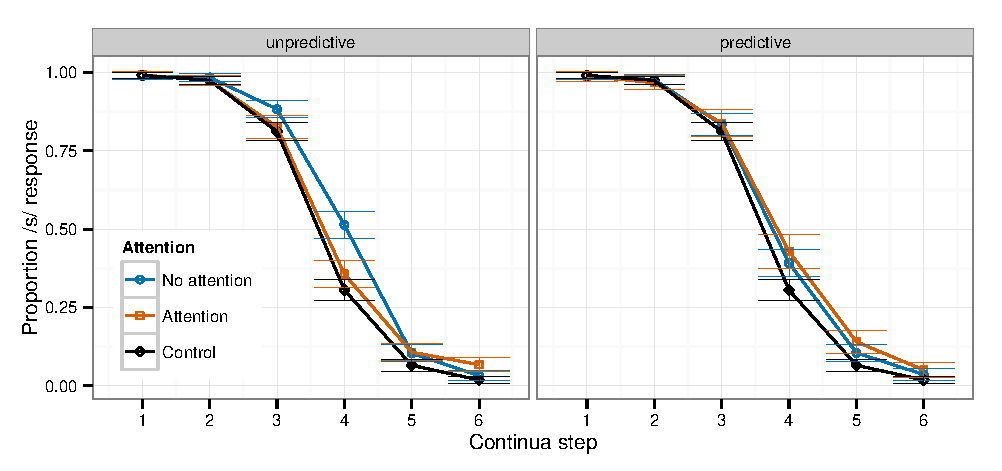
\includegraphics[width=\textwidth]{graphs/exp3_categresults}
\end{center}
\end{figure*}

\section{Discussion}
